\documentclass[13pt, t]{beamer}
% Presento style file
\usepackage{config/presento}

% custom command and packages
% custom packages
\usepackage{textpos}
\setlength{\TPHorizModule}{1cm}
\setlength{\TPVertModule}{1cm}

\newcommand\crule[1][black]{\textcolor{#1}{\rule{2cm}{2cm}}}



\usepackage{color, colortbl}
\setlength{\columnseprule}{0.4pt} 

\title{\Large \hspace{-0.5cm} Comparing phonological systems and syllable structure \\ of Botlikh and Zilo Andi: a data-driven analysis}
\author[shortname]{George Moroz}
\institute[shortinst]{Linguistic Convergence Laboratory, NRU HSE, Moscow, Russia}
\date{\begin{center} {\large 24 October 2019} \bigskip \\ {``Caucasian Languages: Typology and Diachrony'' in honor of M. E. Alekseev, \\ Institute of Linguistics RAS, Moscow}\\ \vfill Presentation is available here: {\large \href{https://tinyurl.com/y5xoks3l}{https://tinyurl.com/y5xoks3l} \hfill 
\includegraphics[height = 2.5cm]{images/01_qrcode}} \end{center}}

\begin{document}

\begin{frame}[plain]
\maketitle
\end{frame}

\begin{frame}[c]{Phonological description: data-driven analysis}
\begin{tabular}{ll|l}
  & \multicolumn{1}{c|}{\textbf{Traditional analysis}} & \multicolumn{1}{c}{\textbf{Data-driven analysis}}                                                                    \\ \hline \pause
1. & Done by trained linguist                          & Evaluated by trained linguist                                                                                       \\ \hline
2. & Could be done from scratch                        & \begin{tabular}[c]{@{}l@{}}A previous description needed\\ (or at least prior expectations)\end{tabular} \\ \hline
3. & Doesn't care about amount of data                 & Care more about amount of data\\ \hline
4. & Less reproducible                 & More reproducible \\ \hline
5. & Could not be automated & Could be automated  
\end{tabular}
\vfill \pause
Data-driven approach to phonological description and syllable structure analysis:
\begin{itemize}
\item was proposed in \citep{moroz2018}
\item was applied to syllable structure  in \citep{moroz2019} to Adyghe data
\item was applied to syllable structure in \citep{romanova2019} to Russian and Macedonian data
\end{itemize} 
\vfill \pause
I will present an application of this method to Botlikh and Zilo Andi data
\end{frame}

\framepic{images/04_map}{\vspace{-0.2cm} Andi and Botlikh villages, created with lingtypology package \citep{moroz2017}}

\begin{frame}
\begin{multicols}{2}
\begin{itemize}
    \item Botlikh < Andic group < EC
    \item Unwritten (can be written with extended Cyrillic script for Avar)
    \item \textasciitilde{}5,000--8,000 speakers
    \item Mostly spoken in 3 villages in northwestern Daghestan (Russian Federation): Botlikh, Miarso, Ashino, (Ankho); minor dialectal differences
    \item One full reference grammar in Georgian  \citep{gudava1962}
    \item Two dictionaries: \\
    \citep{saidovaabusov2012}, \citep{alekseev2019}
\end{itemize}
\vfill
\columnbreak
\begin{itemize}
    \item Andi < Andic group < EC
    \item Unwritten (can be written with extended Cyrillic script for Avar)
    \item \textasciitilde{}16,500 speakers
    \item About 14 villages; There are two main dialect groups: Lower Andi (Muni, Kvankhidatli) and Upper Andi (the rest)
    \item Several reference grammars \citep{suleymanov57} (Rikvani), \citep{salimov10} (Gagatli), \citep{tsertsvadze65} (Andi)
    \item No dictionary except\\ \citep{kibrik1988}
\end{itemize}
\end{multicols}
\end{frame}

\begin{frame}{Comparing two Botlikh dictionaries}

\begin{block}{\citep{saidovaabusov2012}}
    \begin{itemize}
        \item Compiled in the 2000s by a native speaker (M. G. Abusov) and an experienced linguist (P. A. Saidova)
        \item Mostly Botlikh with some notes on Miarso
    \end{itemize}
\end{block}
\pause
\begin{block}{\citep{alekseev2019}}
    \begin{itemize}
        \item Compiled in the 1960s / 1970s by a native speaker / philologist (X. G. Azaev) and later (in the 2000s) systematized by an experienced linguist (M. E. Alekseev)
        \item Subsequently edited by T. A. Maisak and scheduled for posthumous publication later this year
        \item Botlikh only 
    \end{itemize}
\end{block}
\end{frame}

\begin{frame}{Comparing two Botlikh dictionaries}
\begin{block}{Summary:}
\begin{itemize}
\item Dictionaries were compiled \textbf{independently} of each other 
\item with no metadata on the speakers consulted 
\item data collection was separated with several decades break
\end{itemize}
\end{block}
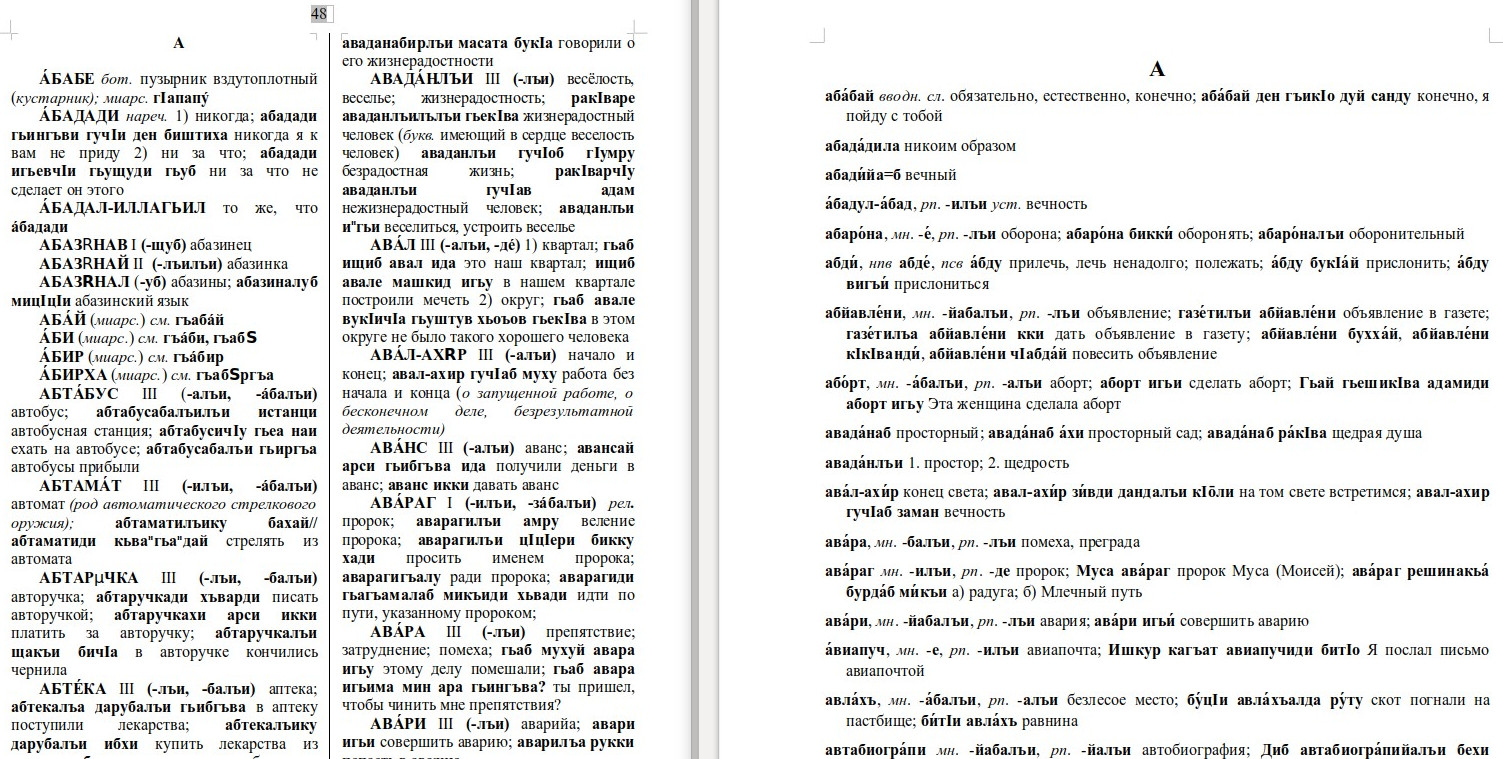
\includegraphics[width=\linewidth]{images/05_dicts}
\end{frame}

\framepic{images/05_dicts}{\begin{itemize}
\item Automatically merge two .doc file into one unified .xls file, ... \pause
\item Manually check for similarities (S. Verhees, C. Naccarato and me)
\end{itemize}
}

\begin{frame}{Comparing two Botlikh dictionaries}
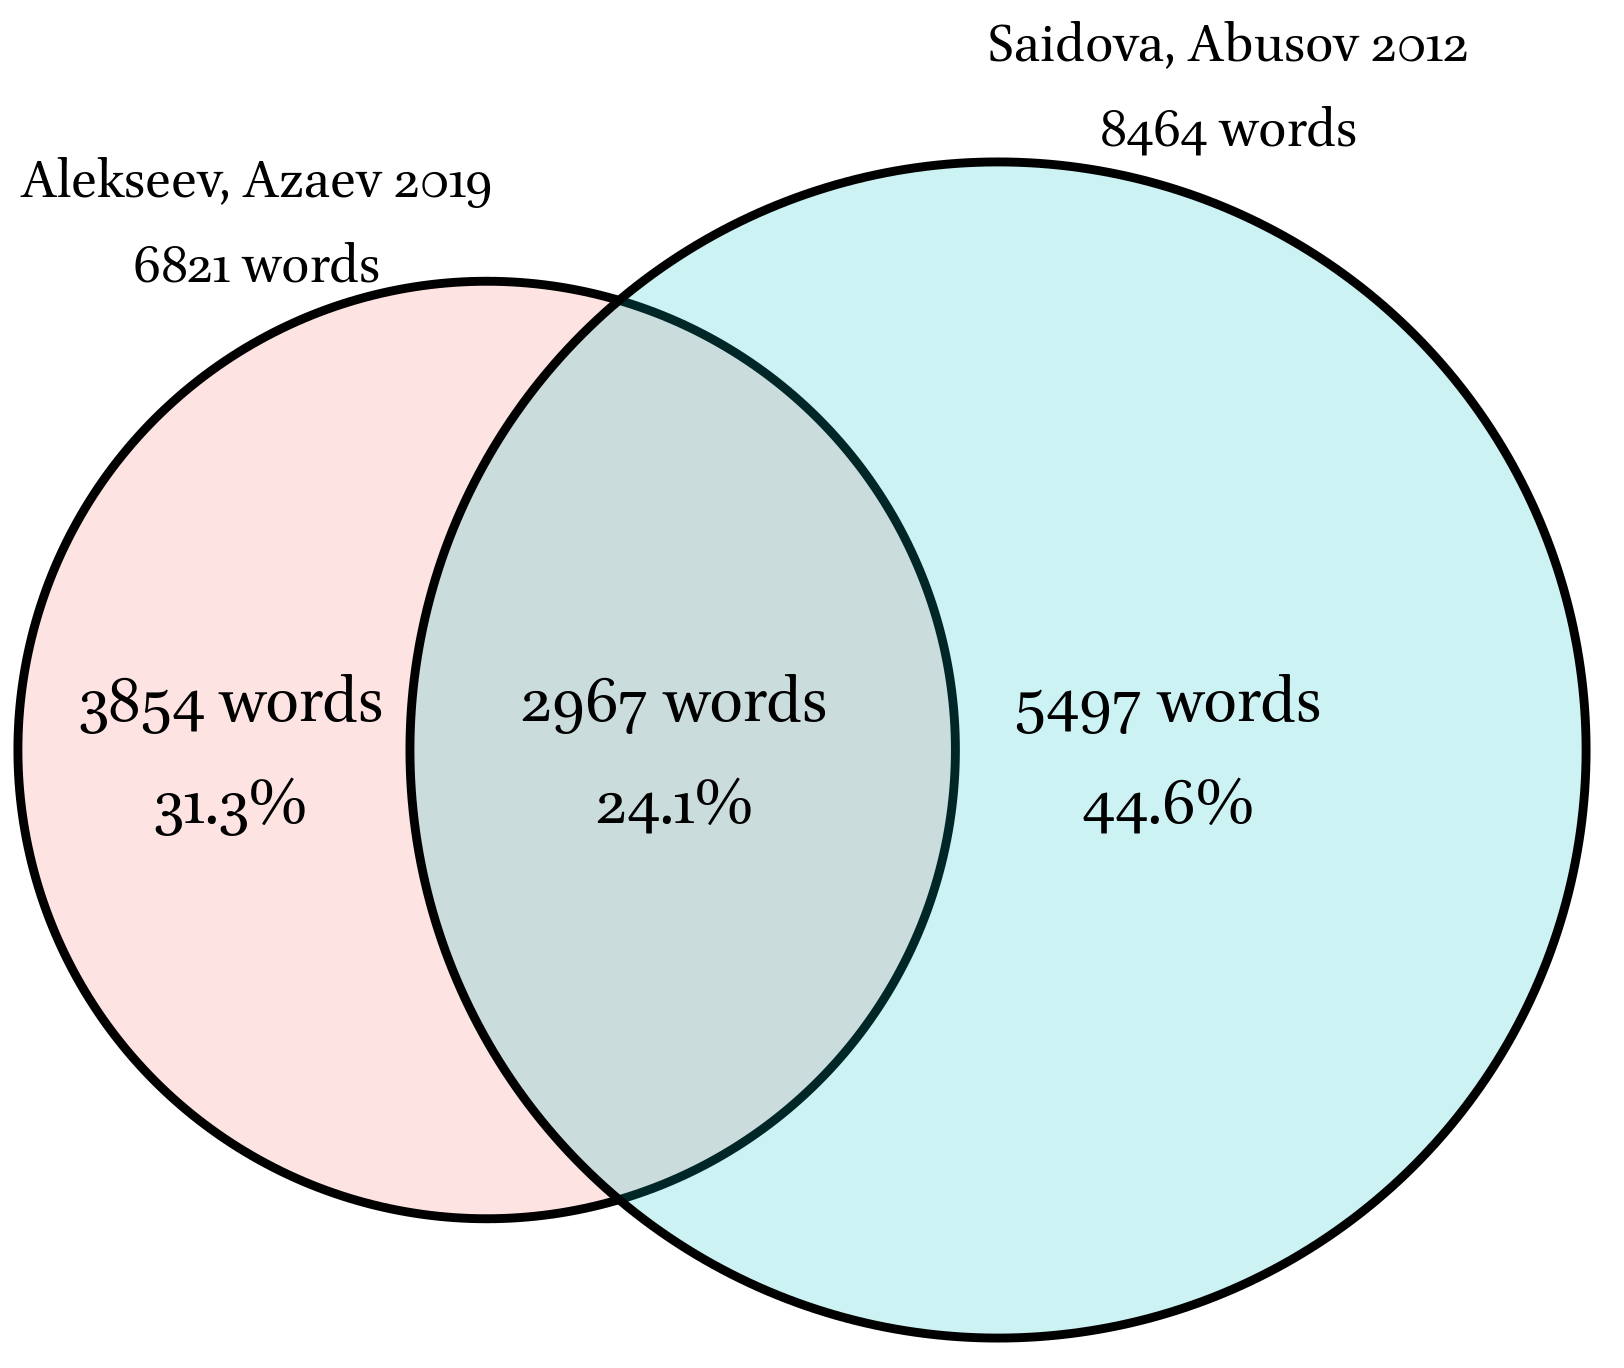
\includegraphics[width=0.94\linewidth]{images/03_venn}
\end{frame}

\begin{frame}{Comparing two Botlikh dictionaries}
\begin{itemize}
\item If we remove a stress sign then there is 2495 same words and 395 different words (14\%)
\item If we don't remove a stress sign then there is 2027 same words and 863 different words (30\%)
\item[\color{colorblue} $\Rightarrow$] There are 16\% of words have different stress pattern?\pause\ Including cases when stress is present in one dictionary and absent in the other. \pause 
\item What cause the difference between dictionaries?
\begin{itemize}
\item Stress pattern differences in 317 words (about 11\%)
\item Multiple cases where there is a small difference that could be explained either as a typo or in terms phonological variation \\ 
\hspace{-5em}\textit{čuhí}~`to~run’~\citep{alekseev2019}  vs. \textit{čũhí} \citep{saidovaabusov2012}, \\
\hspace{-5em}\textit{kusu} `cherry plum’ \citep{alekseev2019}  vs. \textit{kusːu} \citep{saidovaabusov2012}
\item Multiple cases where Russian borrowings were adopted differently \\ 
\hspace{-5em}\textit{awtobus} `bus’ \citep{alekseev2019} vs. \textit{abtabus} \citep{saidovaabusov2012}, \\
\hspace{-5em}\textit{biton} `milk can’ \citep{alekseev2019}  vs. \textit{bitun}~\citep{saidovaabusov2012}, \\
\hspace{-5em}\textit{apteka} `pharmacy’ \citep{alekseev2019} vs. \textit{abteka}~\citep{saidovaabusov2012}
\item Morphological preferences \\
\hspace{-5em}\textit{dinija=w} `pious \citep{alekseev2019} vs. \textit{dinija=b}~\citep{saidovaabusov2012} 
\end{itemize}
\end{itemize}
\end{frame}

\begin{frame}{Comparing two Botlikh dictionaries}
About 25 cases:\\

\begin{tabular}{lll}
\citep{alekseev2019} &\citep{saidovaabusov2012} & \\
\textit{ãha\textbf{\underline{j}}r}   & \textit{ãhar}   & 'message’        \\
\textit{beʒa\textbf{\underline{j}}r}   & \textit{beʒir}   & 'roasting’       \\
\textit{mik'ku\textbf{\underline{j}}r} & \textit{mik'ːur} & 'swallowing’     \\
\textit{reqχu\textbf{\underline{j}}r}  & \textit{reqχʷir} & 'fight’          \\
\textit{reʃku\textbf{\underline{j}}r}  & \textit{reʃkur}  & 'overnight stay’ \\
\textit{rikʷa\textbf{\underline{j}}r}  & \textit{rikʷar} & 'lighting’     \\ \hline
\textit{χwardar} & \textit{χwardir} & 'digging' \\
\textit{miʔar} & \textit{miʔar} & 'nose'\\ 
\dots & \dots & \dots \\ 
& & \\
About 6 cases: & & \\
\textit{ʃːalaj} & \textit{ʃːallaj} & 'silt' \\
\textit{inuʕala} & \textit{inuʕalla} & 'everywhere' \\
\textit{ʕila} & \textit{ʕilla} & 'reason' \\
\dots & \dots & \dots \\
\end{tabular}
\end{frame}

\framepic{images/06_botlikh_dicts_without_stress}{}

\framepic{images/07_botlikh_dicts_with_stress}{}

\begin{frame}
\begin{block}{Conclusions:}
\begin{itemize}
\item Data-driven approach
\end{itemize}
\end{block}
\begin{block}{Discussion:}
\begin{itemize}
\item Botlikh dictionaries were specially selected to share the meaning, the same procedure for Andic were not done
\item Botlikh dictionaries contain a lot of borrowings, it is not true for the Andic dictionary
\item Lemmata are not the same as wordforms, so gathered model should be checked with the wordform material
\item Lemmata could contain some affix that will shift all frequencies (e.~g.~\textsc{inf} or \textsc{pl}) for some types of phonological units
\item It is nice to compare obtained models with the models built on corpora data
\end{itemize}
\end{block}
\end{frame}


\framecard[colorblue]{{\color{colorwhite} \Large Send me a letter!\\
agricolamzgmail.com\\ 
\vfill Presentation is available here: \\tinyurl.com/y3wtkcbq\\
\vfill 
\includegraphics[height = 4cm]{images/02_qrcode}}}

\begin{frame}{References}
\footnotesize
\bibliographystyle{config/chicago}
\bibliography{bibliography}
\end{frame}

\end{document}
